\chapter{Conclusione}

Il campo della predizione della struttura di proteine è stato rivoluzionato nel 2020 grazie allo sviluppo di AlphaFold2 da parte di DeepMind. Il rilascio al pubblico del codice di AlphaFold2 significa che predire la struttura di una proteina a partire dalla sua sequenza amminoacidica è, nella maggior parte dei casi, un problema risolto. Questo non vuol dire che le predizioni siano perfette o che non vi siano famiglie predette in modo poco accurato. AlphaFold2 si rivela tuttavia uno strumento fondamentale poiché permette al mondo della ricerca di ottenere informazioni strutturali su una sequenza di amminoacidi economicamente ed in poche ore.

\par AlphaFold2 non rivoluziona scoprendo un nuovo principio correlato al protein folding. Il segreto dietro al suo successo è un altissimo livello di ingegneria nel deep learning, sfruttando fino all'ultima goccia la mole di conoscenze disponibili sulla struttura delle proteine. La rivoluzione di AF2 è importante anche per le considerazioni sulla ricerca che innalza.

\section{Sfide aperte}

Il problema del \textit{protein folding} non è risolto. È stato risolto, parzialmente, solo il problema della predizione della struttura di proteine.

\subsubsection{Limiti di AlphaFold}
Le predizioni di AF2 sono ragionevoli anche per alcuni casi molto complicati, come proteine ideate e anticorpi, dove i MSA non sono sempre informativi. Tuttavia AlphaFold2 non predice sempre in modo accurato (vedi fig. \ref{fig:af-basso}, dove più del 15\% delle predizioni su nuove strutture nel PDB ha un'accuratezza inferiore agli 8 \angstrom). Nonostante la predizione di AF2 risulti robusta anche in caso di assenza di template e di MSA poco profondi, non risulta altrettanto robusta su MSA quasi interamente non informativi (ad es. composti di 1 o 2 sequenze). 

\begin{figure}[!htb]
	\centering
	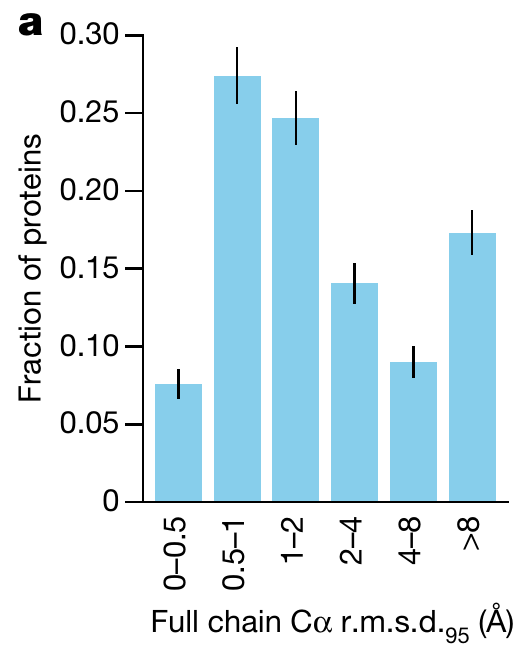
\includegraphics[scale=0.4]{images/af-basso.png}
	\caption{Accuratezza di AF2 su strutture recenti nel PDB. Istogrammi del backbone RMSD per catene intere, sono escluse le proteine con un template dal training set con più del 40\% di identità di sequenza (n=3.144). Fonte\cite{jumper2021highly}}
	\label{fig:af-basso}
\end{figure}

È importante notare che il PDB, ovvero il training set di AlphaFold, ha un forte bias verso le proteine facilmente cristallizzabili: alcune famiglie di proteine sono sottorappresentate e ciò di conseguenza influenza il comportamento predittivo di AlphaFold. Sono osservazioni come questa che alzano questioni sull'eccessiva centralità dei dati nella ricerca scientifica (ricerca definita appunto (\textit{data-centric})).

\subsubsection{Scenari futuri}

L'applicazione più diretta di AF2 è probabilmente il \textit{drug discovery} basato sulla struttura. Fino a prima di AF2 la disponibilità di strutture era un requisito fondamentale: senza di esse non si sarebbe neanche cominciato un progetto. Isomorphic Labs, la nuova società di Demis Hassabis, si basa sugli avanzamenti di AlphaFold per reimmaginare il processo di \textit{drug discovery}.

\par L'ingegneria genetica può essere impiegata per produrre nuove proteine ed enzimi che contengono nuove strutture o svolgono compiti insoliti: metabolizzare rifiuti tossici o sintetizzare farmaci salvavita, ad esempio. La maggior parte dei catalizzatori sintetici non sono paragonabili, in quanto ad efficacia nella capacità di accelerare la velocità di reazioni chimiche selezionate, rispetto agli enzimi naturali. Mentre la conoscenza su come le proteine e gli enzimi sfruttino le loro conformazioni uniche per svolgere le loro funzioni biologiche cresce sempre di più, la capacità di creare nuove proteine con funzioni utili non può che migliorare\supercite{alberts2018essential}.

\par Un'altra applicazione è invece il \textit{protein design}. Il numero di possibili proteine è astronomico e le proteine presenti in natura non sono che una piccolissima frazione di quelle generabili. Per ideare una proteina con una funzione specifica si pensa sia necessario assicurarsi che questa si ripieghi strettamente in una struttura particolare. Finora questo processo è stato rallentato dal tempo necessario per completare un ciclo di design, espressione e determinazione della struttura. Tuttavia, se le previsioni della struttura delle proteine fossero sufficientemente buone da confermare la topologia di una proteina senza una conferma sperimentale, ciò potrebbe accelerare il ciclo di test. \\

\par Per quanto riguarda il mondo della ricerca, in particolare della bioinformatica strutturale, AF2 lo ha liberato del problema del PSP. In questo campo ci si potrà ora dedicare ad altri problemi ancora più importanti e che finora non hanno ricevuto abbastanza attenzione. Degli ambiti di ricerca ora più accessibili sono:

\begin{itemize}
	\item \textit{protein function prediction} 
	\item \textit{predizione delle varianti}
	\item \textit{protein dynamics}, folding e misfolding, aggregazione, regolazione allosterica, flessibilità, disordine delle proteine, fold-switching, ecc.
	\item \textit{binding}, ligandi, interazioni fra proteine, interazioni fra proteine e acidi nucleici, docking macromolecolare, ecc.
\end{itemize}

È possibile che AF2 possa essere trasformativo al punto da essere per le strutture ciò che il sequenziamento del DNA è stato per la genomica. Ogni questione biologica, da quelle molecolari a quelle cellulari, potrebbe essere ora posta in termini di ipotesi strutturali, e ciò potrebbe dar vita ad un nuovo campo come la \textit{structural systems biology}\supercite{moalqAF2}. \\

\section{Etica della ricerca}

\subsubsection{Come è stato possibile realizzare AlphaFold}
{
Ci sono vari motivi di contorno al successo di DeepMind che hanno portato questo gruppo a sviluppare un sistema software in grado di risolvere il problema della predizione della struttura di proteine. È possibile elencare almeno 3 motivi principali:

\begin{itemize}
	\item capacità del team e velocità di comunicazione
	\item potenza computazionale senza limiti
	\item tanti dati e conoscenza dalla ricerca
\end{itemize}

Prima di tutto c'è il gruppo di ricerca in sé organizzato da DeepMind. Oltre alle competenze dimostrate, un gruppo di ricerca privato ha la possibilità di sperimentare e scambiarsi idee e informazioni molto più velocemente dei gruppi accademici. L'organizzazione è differente, così come gli obiettivi a lungo termine. Il paradigma di lavoro nella ricerca privata si può definire di tipo \textit{fast and focused}. Il motivo per cui il paper di AlphaFold ha circa 20 coautori principali è che tutti vanno nella stessa direzione.

\par C'è poi anche l'aspetto della (praticamente) illimitata potenza computazionale a disposizione. Nonostante possa forse aver accelerato i tempi di sperimentazione, la potenza a disposizione è solo un elemento di contorno per il raggiungimento dell'alto livello ingegneristico di AlphaFold.

\par DeepMind afferma di aver utilizzato approssimativamente 128 TPUv3 core in funzione per varie settimane, una quantità di risorse non eccessiva nel panorama attuale dello stato dell'arte del ML. Le TPU sono state sviluppate da Google appositamente per il deep learning e nelle giuste mani possono mostrare la loro marcia in più. Una tra le loro caratteristiche più importanti è la quantità di memoria: un chip 8-core TPUv3 ha 128 GB di vRAM, dove invece le comuni GPU arrivano a circa 40-80 GB. Il costo di noleggio annuale di 128 TPU può aggirarsi intorno al milione di dollari\supercite{blopigAF}.

\par I gruppi Baker e Zhang, i migliori dopo AlphaFold nel CASP14, per confronto hanno riferito di avere usato 4 GPU per allenare i loro modelli per un paio di settimane. Ciò che per questi due gruppi richiede un mese di sperimentazione potrebbe richiedere solo qualche ora per DeepMind. È quindi giusto considerare questo fattore come un vantaggio, che consente sia un efficace \textit{rapid prototyping} per testare varie idee, che una base solida su cui poggiare un'architettura come quella di AlphaFold.\\


\par Un motivo invece più interessante da sottolineare è l'enorme quantità di dati e conoscenze prodotti e pubblicati dai gruppi accademici di ricerca negli ultimi decenni. AlphaFold, come tutti i sistemi di ML, può funzionare grazie alla presenza di grandi quantità di dati (milioni di sequenze e migliaia di strutture) e grazie alla conoscenza scientifica nel settore. Spesso la precedente ricerca è stata possibile grazie a fondi pubblici o iniziative accademiche finanziate dai governi, come i tool HHblits, JackHMMER e OpenMM usati da AF2. In altre parole, DeepMind è riuscita a vedere lontano e a realizzare AlphaFold perché si trova sulle \textit{spalle di giganti}.

\subsubsection{Ricerca accademica e industriale}

 \par Il raggiungimento di DeepMind può essere visto come un'accusa nei confronti del mondo accademico. Per un lungo periodo se si voleva fare ricerca e risolvere problemi di ricerca (come il PSP) il percorso che si delineava era trovare un lavoro nel sistema accademico. Oggi, nel 2022, la differenza è che l'industria non è più solo un buon posto per fare ricerca applicata ma potrebbe diventare un posto dove fare quasi esclusivamente tutta la ricerca applicata. Tuttavia ci sono alcune considerazioni da fare per rendersi conto di cosa comporterebbe una tale prospettiva.

\par L'ultimo punto citato nella sezione precedente è particolarmente interessante poiché ci si può chiedere: se si vuole che la scienza rimanga aperta e collaborativa, fino a che punto l'informazione creata da centri di ricerca pubblici (pubblici al fine di stimolare ulteriore ricerca) appartiene alla comunità e sotto quali condizioni potrebbe essere usata per iniziative for-profit?\supercite{blopigAF} In questo caso DeepMind ha preso la decisione di condividere al pubblico il codice di AlphaFold e di rendere lo strumento apertamente accessibile. Ma al di fuori del caso specifico, l'interrogativo rimane, specialmente con l'avvento della ricerca \textit{data-centric}, basata sui dati e sull'intelligenza artificiale.

\par Riguardo allo sbilanciamento nelle risorse computazionali, una domanda che sorge è se questo impatterà la qualità della ricerca accademica in futuro. I modelli si stanno facendo sempre più complessi (vedi transformer) e la complessità cresce più di quanto cali il prezzo dell'hardware. Si potrebbe arrivare alla situazione poco sensata nella quale la ricerca accademica sia limitata  a raggiungere le idee che vorrebbero inseguire dalla mancanza di disponibilità computazionale. 

\par Per ovviare a tale problema si possono immaginare vari scenari\supercite{blopigAF}:
\begin{itemize}
	\item i gruppi di ricerca ricevono significativi investimenti nelle infrastrutture perché viene compreso il vantaggio che strumenti come AlphaFold potrebbero apportare
	\item le risorse di ricerca potrebbero essere condivise in un consorzio internazionale, come i fisici delle alte energie hanno fatto per il CERN
	\item si segue la strada di sviluppare strategie per ridurre l'impatto delle risorse limitate sugli strumenti di ML; ci sarebbe bisogno di più software engineer professionisti di alto livello
\end{itemize}

Il paradigma \textit{fast and focused} dei centri di ricerca privati come DeepMind ha però dei vincoli, ad esempio\supercite{moAlq}:
\begin{itemize}
	\item non pone nuove domande
	\item fa fiorire una sola idea
\end{itemize}

 È un approccio ottimo per rispondere a delle domande precise, ma non per porre domande. Nel mondo biologico e scientifico in generale, definire domande è una parte importante del lavoro di ricerca. Non è un lavoro banale riuscire a strutturare una competizione scientifica come il CASP, e se è stato fatto è grazie allo sforzo collettivo di tanti membri della comunità scientifica. DeepMind infatti si concentra su problemi con obiettivi e metriche chiare, non sulla definizione di nuove domande.

\par  Nonostante il paper di AF2 sia stato pubblicato, compresi alcuni studi di ablazione, internamente DeepMind potrebbe aver provato molti altri approcci ma solamente quelli vincenti vengono esplorati e condivisi. È però possibile che quei percorsi scartati, pur non contribuendo direttamente alla soluzione, avrebbero potuto produrre altri tipi di conoscenza riguardo al problema. Il paradigma in questione minimizza la circolazione ed esplorazione di idee. Non è un problema specifico di DeepMind ma di come si sta evolvendo la ricerca in sé, specialmente nel caso del ML.
 
 \par Infine un'osservazione sul confronto fra ricerca accademica e industriale riguarda il livello di interessi nelle questioni pubbliche. Immaginando di dover convocare un consiglio speciale di esperti di un settore (es. epidemiologia, intelligenza artificiale) non ci si può aspettare che convocando membri di grandi aziende questi non abbiano degli interessi personali.

}

\clearpage
